\chapter{Название главы}
\section{Название секции}

Внутритекстовая формула $\frac{1}{\epsilon^*}=\frac{1}{\epsilon_\infty}-\frac{1}{\epsilon_0}$.
Внутритекстовая формула в стиле выделенной $\dfrac{1}{\epsilon_\infty}$.
Ссылки на литературу~\cite{Yoffe_1993_AP_42_173,Efros_1982_FTP_16_7_1209,%
Anselm_1978,Segall_1968,Agranovich_1983,InP,Mishchenko_1996,Skvortsov_2008,%
Perelman_2003_math:0307245,Nielsen_2010_1006.2735,patent1,patent2}. Ссылка на формулу~\eqref{e:Coulomb}
\begin{equation}\label{e:Coulomb}
  \frac{1}{|\vec r_1 - \vec r_2|} =
  4\pi \int \frac{d^3 q}{(2\pi)^3}\,
  \frac{e^{i\vec q(\vec r_1 - \vec r_2)}}{q^2}.
\end{equation}

Ссылка на рис.~\ref{f:fig}
\begin{figure}[!ht]
  \centering
  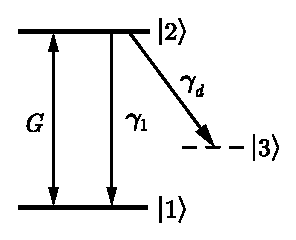
\includegraphics[width=4cm]{fig}
  \caption{\label{f:fig}%
  Подпись к рисунку.
  }
\end{figure}

\begin{wrapfigure}{r}{0.35\textwidth}
\centering
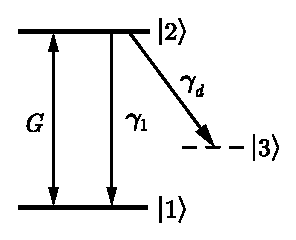
\includegraphics[width=4cm]{fig}
\caption{\label{f:ff}%
Рисунок <<в оборку>>.
}
\end{wrapfigure}

Если разность энергий электронно-дырочных уровней $E_2 - E_1$ близка к энергии продольного оптического фонона $\hbar\Omega_{\mathrm{LO}}$, то в разложении волновых функций полного гамильтониана можно ограничиться нулевым приближением для всех состояний, за исключением близких по значению к $E_2$.
Волновые функции последних представляют собой следующие комбинации вырожденных состояний\footnote{Текст сноски}.

Ссылка на таблицу~\ref{t:InPSiO2}.
\begin{table}[!ht]
  \centering
  \caption{Пример таблицы}\label{t:InPSiO2}
  \begin{tabular}{l|ccc}
    \hline\hline
    & \quad$\lambda \cdot 10^{-11}$,~$\text{дин}\cdot\text{см}^{-2}$
    & \quad$\mu \cdot 10^{-11}$,~$\text{дин}\cdot\text{см}^{-2}$
    & \quad$\rho$, $\text{г}\cdot\text{см}^{-3}$ \\
    \hline
    InP       & 3.82 & 1.69 & 4.14 \\
    SiO$_{2}$ & 1.57 & 3.11 & 2.2  \\
    \hline\hline
  \end{tabular}
\end{table}

\begin{figure}[!ht]
  \centering
  \begin{minipage}{5cm}
    \centering
    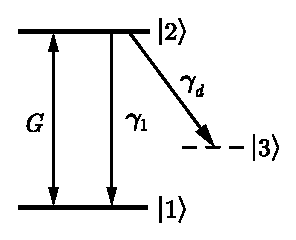
\includegraphics[width=4cm]{fig}
    \caption{Рисунок с отдельным названием}
  \end{minipage}
  \quad
  \begin{minipage}{5cm}
    \centering
    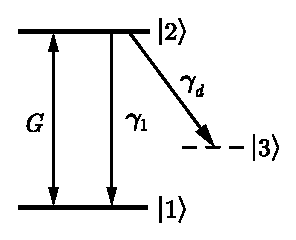
\includegraphics[width=4cm]{fig}
    \caption{Рисунок с отдельным названием}
  \end{minipage}
  \quad
  \begin{minipage}{5cm}
    \centering
    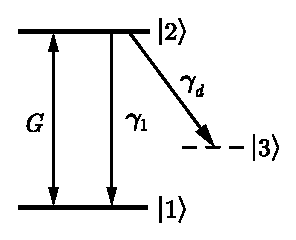
\includegraphics[width=4cm]{fig}
    \caption{Рисунок с отдельным названием}
  \end{minipage}
\end{figure}

\begin{figure}[!ht]
  \centering
  \begin{minipage}{5cm}
    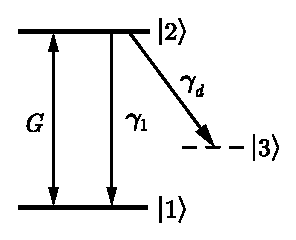
\includegraphics[width=4cm]{fig}
  \end{minipage}
  \begin{minipage}{5cm}
    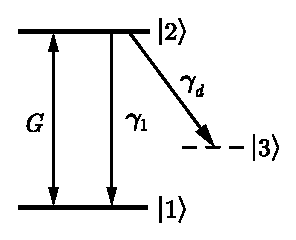
\includegraphics[width=4cm]{fig}
  \end{minipage}
  \caption{Рисунки с единым названием}
\end{figure}

Ссылка на внутренний рисунок (рис.~\ref{f:sub1}).

\begin{figure}[!ht]
\centering
  \begin{minipage}{5cm}
    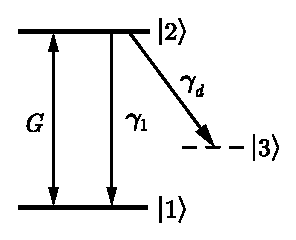
\includegraphics[width=4cm]{fig}\subcaption{}\label{f:sub1}
  \end{minipage}
  \begin{minipage}{5cm}
    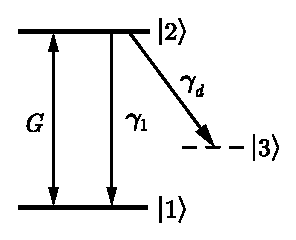
\includegraphics[width=4cm]{fig}\subcaption{}\label{f:sub2}
  \end{minipage}
  \begin{minipage}{5cm}
    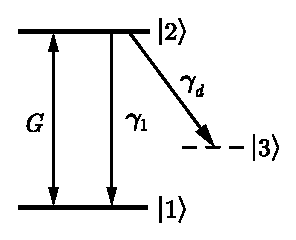
\includegraphics[width=4cm]{fig}\subcaption{}\label{f:sub3}
  \end{minipage}
  \caption[]{%
  Рисунки с единым названием и подчиненной нумерацией:
    \subref{f:sub1} ссылка 1,
    \subref{f:sub2} ссылка 2,
    \subref{f:sub3} ссылка 3.
  }
\end{figure}

\subsection{Название подсекции}
Текст подсекции
\subsubsection{Название под-подсекции}
Текст под-подсекции
\paragraph{Название параграфа.}
Текст параграфа
\subparagraph{Название подпараграфа.}
Текст подпараграфа

Нумеруемый список:
\begin{enumerate}
  \item Первый уровень вложенности.
  \begin{enumerate}
    \item Второй уровень вложенности.
    \begin{enumerate}
      \item Третий уровень вложенности.
    \end{enumerate}
  \end{enumerate}
\end{enumerate}

Демонстрация полностью настраиваемых окружений типа <<теорема>>.

\newtheorem{theorem}{Теорема}[chapter]
\def\theoremstyle{}
\def\postthetheorem{:}

\newtheorem{lemm}{Лемма}[chapter]
\def\thelemmstyle{\bfseries}
\def\oparglemmstyle{}
\def\lemmstyle{}
\def\preoparglemm{(}
\def\postoparglemm{):}

\newtheorem{remark}{Примечание}[chapter]
\def\remarkstyle{\itshape}
\def\theremarkstyle{}
\def\posttheremark{:}

\begin{lemm}[Шура]
Квадратная матрица, коммутирующая со всеми матрицами неприводимого представления, кратна единичной.
\end{lemm}

\begin{theorem}
Гомоморфный образ группы изоморфен фактор-группе по ядру гомоморфизма.
\end{theorem}

\begin{remark}
Текст примечания.
\end{remark}
